\documentclass[12pt]{article}
\usepackage{amsmath, amsthm, amssymb}
\usepackage{hyperref}
\usepackage{verbatim}
\usepackage[top=1.0in, bottom=1.0in, left=1.0in, right=1.0in]{geometry}

\pagestyle{plain}

\usepackage{tkz-graph}
\usetikzlibrary{arrows}
\usetikzlibrary{shapes}
\usepackage[position=bottom]{subfig}

\usepackage{longtable}
\usepackage{array}

\usepackage{sectsty}
\allsectionsfont{\sffamily}

\setcounter{secnumdepth}{5}
\setcounter{tocdepth}{5}

\makeatletter
\newtheorem*{rep@theorem}{\rep@title}
\newcommand{\newreptheorem}[2]{
\newenvironment{rep#1}[1]{
 \def\rep@title{#2 \ref{##1}}
 \begin{rep@theorem}}
 {\end{rep@theorem}}}
\makeatother

\theoremstyle{plain}
\newtheorem{thm}{Theorem}[section]
\newreptheorem{thm}{Theorem}
\newtheorem{prop}[thm]{Proposition}
\newreptheorem{prop}{Proposition}
\newtheorem{lem}[thm]{Lemma}
\newreptheorem{lem}{Lemma}
\newtheorem{conjecture}[thm]{Conjecture}
\newreptheorem{conjecture}{Conjecture}
\newtheorem{cor}[thm]{Corollary}
\newreptheorem{cor}{Corollary}
\newtheorem{prob}[thm]{Problem}
\newtheorem{observation}{Observation}
\newtheorem*{mainconj}{Main Conjecture}
\newtheorem*{mainthm}{Main Theorem}

\theoremstyle{definition}
\newtheorem{defn}{Definition}
\theoremstyle{remark}
\newtheorem*{remark}{Remark}
\newtheorem*{problem}{Problem}
\newtheorem{example}{Example}
\newtheorem*{question}{Question}


\newcommand{\fancy}[1]{\mathcal{#1}}
\newcommand{\C}[1]{\fancy{C}_{#1}}
\newcommand{\IN}{\mathbb{N}}
\newcommand{\IR}{\mathbb{R}}
\newcommand{\G}{\fancy{G}}
\newcommand{\CC}{\fancy{C}}
\newcommand{\D}{\fancy{D}}

\newcommand{\inj}{\hookrightarrow}
\newcommand{\surj}{\twoheadrightarrow}

\newcommand{\set}[1]{\left\{ #1 \right\}}
\newcommand{\setb}[3]{\left\{ #1 \in #2 \mid #3 \right\}}
\newcommand{\setbs}[2]{\left\{ #1 \mid #2 \right\}}
\newcommand{\card}[1]{\left|#1\right|}
\newcommand{\size}[1]{\left\Vert#1\right\Vert}
\newcommand{\ceil}[1]{\left\lceil#1\right\rceil}
\newcommand{\floor}[1]{\left\lfloor#1\right\rfloor}
\newcommand{\func}[3]{#1\colon #2 \rightarrow #3}
\newcommand{\funcinj}[3]{#1\colon #2 \inj #3}
\newcommand{\funcsurj}[3]{#1\colon #2 \surj #3}
\newcommand{\irange}[1]{\left[#1\right]}
\newcommand{\join}[2]{#1 \mbox{\hspace{2 pt}$\ast$\hspace{2 pt}} #2}
\newcommand{\djunion}[2]{#1 \mbox{\hspace{2 pt}$+$\hspace{2 pt}} #2}
\newcommand{\parens}[1]{\left( #1 \right)}
\newcommand{\brackets}[1]{\left[ #1 \right]}
\newcommand{\nint}[1]{\widetilde{N}\left(#1\right)}
\newcommand{\DefinedAs}{\mathrel{\mathop:}=}
\newcommand{\pot}{\operatorname{pot}}

\def\adj{\leftrightarrow}
\def\nonadj{\not\!\leftrightarrow}

\def\D{\fancy{D}}
\def\C{\fancy{C}}
\def\Q{\fancy{Q}}
\def\Z{\fancy{Z}}

% any changes to \claim should be mirrored in \claimnonum and \subclaim
\newcommand{\claim}[2]{{\bf Claim #1.}~{\it #2}~~}
\newcommand{\claimnonum}[1]{{\bf Claim.}~{\it #1}~~}
\newcommand{\subclaim}[2]{{\bf Subclaim #1.}~{\it #2}~~}

\begin{document}
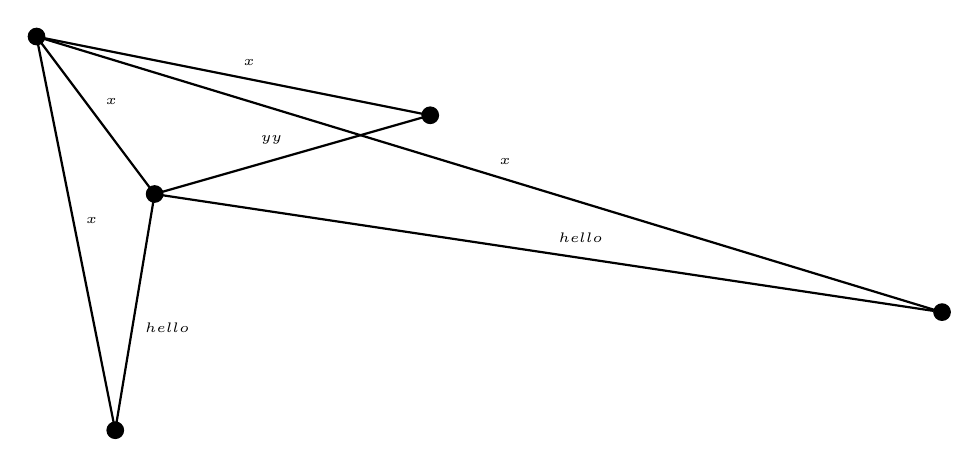
\begin{tikzpicture}[scale = 10]
\tikzstyle{VertexStyle} = []
\tikzstyle{EdgeStyle} = []
\tikzstyle{labeledStyle}=[shape = circle, minimum size = 6pt, inner sep = 1.2pt, draw]
\tikzstyle{unlabeledStyle}=[shape = circle, minimum size = 6pt, inner sep = 1.2pt, draw, fill]
\Vertex[style = unlabeledStyle, x = 0.550000011920929, y = 0.799999997019768, L = \tiny {}]{v0}
\Vertex[style = unlabeledStyle, x = 0.699999988079071, y = 0.599999994039536, L = \tiny {}]{v1}
\Vertex[style = unlabeledStyle, x = 1.04999995231628, y = 0.699999988079071, L = \tiny {}]{v2}
\Vertex[style = unlabeledStyle, x = 1.70000004768372, y = 0.449999988079071, L = \tiny {}]{v3}
\Vertex[style = unlabeledStyle, x = 0.649999976158142, y = 0.300000011920929, L = \tiny {}]{v4}
\Edge[label = \tiny {$yy$}, labelstyle={auto=right, fill=none}](v2)(v1)
\Edge[label = \tiny {$hello$}, labelstyle={auto=right, fill=none}](v3)(v1)
\Edge[label = \tiny {$hello$}, labelstyle={auto=right, fill=none}](v4)(v1)
\Edge[label = \tiny {$x$}, labelstyle={auto=right, fill=none}](v2)(v0)
\Edge[label = \tiny {$x$}, labelstyle={auto=right, fill=none}](v3)(v0)
\Edge[label = \tiny {$x$}, labelstyle={auto=right, fill=none}](v4)(v0)
\Edge[label = \tiny {$x$}, labelstyle={auto=right, fill=none}](v1)(v0)
\end{tikzpicture}

\end{document}
